\documentclass[a4paper,12pt]{article} % тип документа

\newcommand\nameone{Цыганкова Екатерина}
\newcommand\groupone{Б02-409}
\newcommand\labnumber{4.5.2}
\newcommand\labwork{Поляризация}
%%% Работа с русским языком
\usepackage{cmap}					% поиск в PDF
\usepackage{mathtext} 				% русские буквы в формулах
\usepackage[T2A]{fontenc}			% кодировка
\usepackage[utf8]{inputenc}			% кодировка исходного текста
\usepackage[main = russian, english]{babel}	% локализация и переносы
%\selectlanguage{english} (для англостатей)
%\usepackage{caption}

%%% Дополнительная работа с математикой
\usepackage{amsmath,amsfonts,amssymb,amsthm,mathtools} % AMS
\usepackage{icomma}
\usepackage{physics}
\usepackage{multicol}
\usepackage{bm}
\usepackage{mathrsfs}
\usepackage{verbatim}

%%% Номера формул
%\mathtoolsset{showonlyrefs=true} 
%\usepackage{leqno} 

%%% Свои команды
\DeclareMathOperator{\sgn}{sgn}

\usepackage{csquotes} 
\usepackage[backend=biber,style=authoryear]{biblatex}


%%% Работа с графикой
\usepackage{graphicx}
\graphicspath{{images/}}  
\setlength\fboxsep{3pt} 
\setlength\fboxrule{1pt} 
\usepackage{wrapfig} 
\usepackage{subcaption}
\usepackage{tikz}
\usepackage{pgfplots}
\usepackage{pgfplotstable}
\usepgfplotslibrary{polar}
\pgfplotsset{compat=1.18} 

%%% Работа с таблицами
\usepackage{array,tabularx,tabulary,booktabs}
\usepackage{longtable}  
\usepackage{multirow} 
\usepackage{soul} 

%%% Теоремы
\theoremstyle{plain} 
\newtheorem{theorem}{Th}[section]
\newtheorem{proposition}[theorem]{Proposition}
\newtheorem{question}{Question}[section]
 
\theoremstyle{definition} 
\newtheorem{corollary}{Corollary}[theorem]
\newtheorem{problem}{Problem}[section]
\newtheorem{definition}{Def}[section]
 
\theoremstyle{remark} 
\newtheorem*{nonum}{Solution}

%%% Программирование
\usepackage{etoolbox} 

%%% Гиперссылки
\usepackage{hyperref}

\usetikzlibrary{knots}
\usepackage{tcolorbox}

%%% Страница
\usepackage{geometry} 
	\geometry{top=20mm, bottom=20mm, left=15mm, right=20mm}

\usepackage{setspace} 

\usepackage{lastpage} 
\usepackage{amssymb}
\usepackage{xcolor}
\usepackage[all]{xy}
\usepackage{dsfont}



\begin{document}
\begin{center}   
	\large{Лабораторная работа № \labnumber\\ \hfill \break\Large{\textbf{\labwork}}}\\
    \normalsize
    \begin{flushright}
    \nameone, \groupone \\
    \today
    \end{flushright}
\end{center}
\begin{center}
    В работе изучаются свойства лазерного излучения для гелий-неонового лазера на основе резонаторе Фабри-Перо. По изменению видности интерференционной картины, получаемой в интерферометре Майкельсона, изучены поляризация и спектральный состав света, генерируемого лазером. Проведено сравнение полученных результатов с теоретическими оценками. 
\end{center}

\tableofcontents

\newpage

\section{Теоретическое введение}
Гелий-неоновый лазер, используемый в работе, представляет из себя резонатор Фабри-Перо с расстоянием между генерируемыми модами $\delta \nu = \frac{c}{2 L} = 200 \divisionsymbol 300$ МГц ($L = 0,5 \divisionsymbol 0,7$ м -- длина резонатора, $c$ -- скорость света) и спектральной шириной $\sim 10$ МГц. 

Ширина спектра излучения в основном определяется доплеровским уширением $\Delta nu_\text{д} \sim \frac{1}{\lambda_0} \sqrt{\frac{8 R T}{\pi \mu}}$. Для лазерного перехода атома неона с длиной волны $\lambda_0 = 632,8$ нм и $T = 400$ К: $\Delta nu_\text{д} \sim 10^9$ Гц. Таким образом, лазер излучает 3-5 когерентных мод. 
\subsection{Видность интерференционной картины}

Для оценки чёткости интерференционной картины в окрестности некоторой точки используют параметр видности:

\begin{equation}
    V =\frac{I_\text{max} - I_\text{min}}{I_\text{max} + I_\text{min}}~,
\end{equation}

где $I_\text{max}$ и $I_\text{min}$ -- максимальная и минимальная интенсивности света интерференционной картины вблизи выбранной точки. Видность интерференционных картин, получаемых с помощью лазерного излучения зависит от нескольких факторов.

\textbf{1. Отношение интенсивности интерферирующих волн.}

Если на выходе из интерференционной схемы интенсивности двух интерферирующих волн равны соответственно $I_A$ и $I_B$, то видность интерференционной картины равна:
\begin{equation}
    \label{eq:V1}
    \boxed{
    V_1 = \frac{2 \sqrt{I_A I_B}}{I_A + I_B} = \frac{2 \sqrt{\delta}}{1 + \delta}}
\end{equation}

Здесь $\delta \equiv \frac{I_A}{I_B}$.

\textbf{2. Спектральный состав излучения и разность хода интерферирующих волн.}
Рассмотрим случай $I_A = I_B$. Когда в интерференции участвуют несколько спектральных компонент, интенсивности их интерференционных картин складываются:

\begin{equation}
    I = \sum_{\omega \text{-- генерируемые моды}} 2 I_\omega (1 + \cos(\frac{\omega}{c}l)) ~,
\end{equation}
где $l$ -- разность хода между интерферирующими лучами. Видность $V_2$ тогда зависит от разности хода $l$.

В случае интерференции $n$ спектральных мод одинаковой интенсивности с интервалом $\delta \nu = \frac{c}{2 L}$ между ними, видность определяется по формуле:

\begin{equation}
    V_2 = \left|\frac{1}{n} \frac{\sin \frac{\pi l}{2 L}n}{\sin\frac{\pi l}{2 L}}\right|
\end{equation}

В этом случае видность впервые обнуляется при разности хода $l = \frac{2 L}{n} = \frac{c}{\Delta \nu}$ ($\Delta \nu = n \delta \nu$ -- полная ширина спектра).

В общем случае (при других отношениях интенсивностей) зависимость видности $V_2(l)$ может иметь другой вид, но сохраняется связсь геометрической задержки $l_{1/2}$, при которой видность падает вдвое, c полной шириной спектра и количеством мод:

\begin{equation}
    \label{eq:assess}
    \boxed{
    \Delta \nu \sim 0,6 \frac{c}{l_{1/2}} ~~~~~ n \sim 1 + 1,2 \frac{L}{l_{1/2}}}
\end{equation}

\textbf{3. Поляризация интерферирующих пучков.}

Для исследования зависимости видности от поляризации излучения, в работе были установлены поляроиды в каждом из плечей интерферометра. Зависимость видности от угла между поляроидами $\beta$ может принимать две формы. 

Если лазерное излучение имеет постоянную линейную поляризацию, то $V_3 = |\cos \beta|$. Если же линейная поляризация лазерного излучения не постоянна и меняется хаотически от 0 до $\pi$ то $V_3 = \cos^2 \beta$.

Если имеют место все три фактора уменьшения видности, то результирующая видность является произведением:

\begin{equation}
    V = V_1 V_2 V_3
\end{equation}

\section{Экспериментальная установка}

\begin{figure}[h]
    \centering
    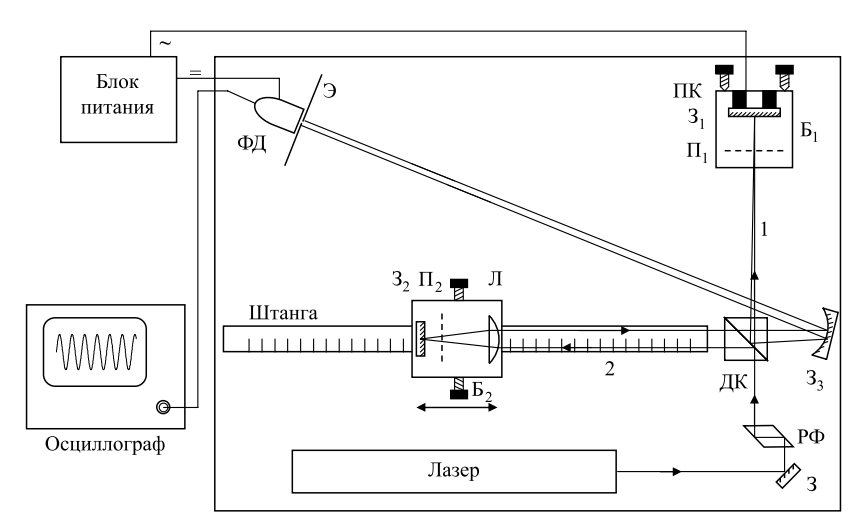
\includegraphics[width = 0.9\textwidth]{pics/setup}
    \caption{Схема установки. З, $\text{З}_1$, $\text{З}_2$, $\text{З}_3$ -- зеркала. $\text{П}_1$ и $\text{П}_2$ -- поляроиды. $\text{Б}_1$ и $\text{Б}_2$ — блоки № 1 и 2. ДК -- делительный кубик, РФ -- ромб Френеля.
ФД -- фотодиод, Э -- экран, ПК -- пьезокерамика, Л -- линза}
\label{fig:setup}
\end{figure}

Для исследования поляризации и спектрального состава излучения гелий-неонового лазера, в работе используется интерферометр Майкельсона (Рис. \ref{fig:setup}). Луч лазера,
отражённый от зеркала З и прошедший через ромб Френеля (РФ), делится
делительным кубиком ДК на два луча. Первый луч проходит блок $\text{Б}_1$ с
поляроидом $\text{П}_1$ и зеркалом $\text{З}_1$, прикленным к пьезокерамике. Пьезокерамика
может совершать малые колебания вдоль луча c частотой много меньшей частоты колебаний волны и амплитудой порядка нескольких длин волн. Второй луч проходит блок $\text{Б}_2$ с линзой Л, поляроидом
$\text{П}_2$ и зеркалом $\text{З}_2$ в фокальной плоскости линзы. Оба луча,
проходя ДК, попадают на сферическое зеркало $\text{З}_3$ и интерферируют на
экране. Через щель в центре экрана, ширина которой значительно меньше расстояния между интерференционными полосами, свет попадает на фотодиод. Интенсивность света пропордиональна напряжению фотодиода, измеряемому осциллографом. 

\begin{wrapfigure}{r}{0.4\textwidth}
    \begin{center}
        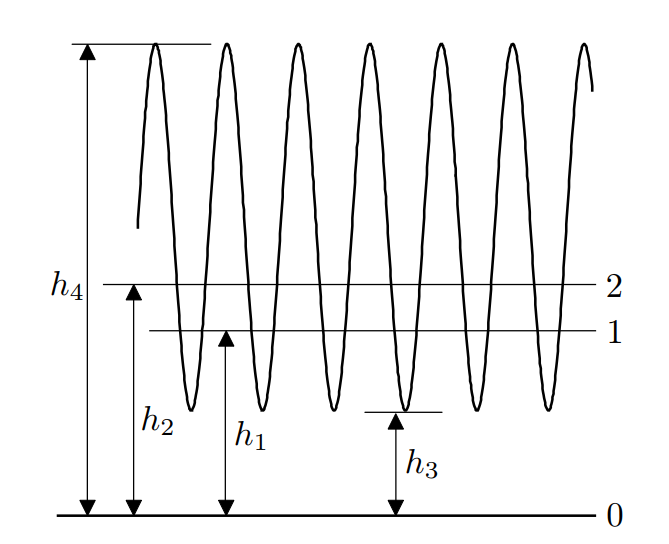
\includegraphics[width = \linewidth]{pics/osc}
    \end{center}
    \caption{Осциллограмма сигналов фотодиода.}
    \label{fig:osc}
\end{wrapfigure}
\vspace{10pt}

По картине на экране осциллографа можно определить параметры видности по следующим формулам:
\begin{equation}
    \label{eq:delta_V}
    \delta = \frac{h_1}{h_2} ~~~~
    V = \dfrac{h_4 - h_3}{h_4 + h_3}
\end{equation}

Здесь 0 -- уровень засветки при отсутствии лучей, 1 и 2 -- при перекрытии одного из них.
Используя $\delta$, можно рассчитать $V_1$ по формуле \eqref{eq:V1}.

При условии одинаковой поляризации лучей ($\beta = 0$),
\begin{equation}
    \label{eq:V2}
    V_2 = \frac{V}{V_1}.
\end{equation}
Если же разность хода отсутствует ($l = 0$), то
\begin{equation}
    \label{eq:V3}
    V_3 = \frac{V}{V_1}.
\end{equation}

\section{Измерение зависимости видности от поляризации}

\begin{wraptable}{r}{0.25\textwidth}
    \centering
    
\begin{tabular}{|c|c|c|}
\hline
\begin{tabular}[c]{@{}c@{}}$\beta, ^\circ$\\ $\sigma_\beta = 1^\circ$\end{tabular} & $V_3$ & $\sigma_{V_3}$ \\ \hline
0.0                                                                                & 0.84  & 0.07           \\ \hline
10.0                                                                               & 0.88  & 0.07           \\ \hline
20.0                                                                               & 0.88  & 0.08           \\ \hline
25.0                                                                               & 0.91  & 0.10           \\ \hline
30.0                                                                               & 0.83  & 0.10           \\ \hline
35.0                                                                               & 0.83  & 0.10           \\ \hline
40.0                                                                               & 0.82  & 0.15           \\ \hline
45.0                                                                               & 0.81  & 0.15           \\ \hline
50.0                                                                               & 0.71  & 0.13           \\ \hline
55.0                                                                               & 0.66  & 0.06           \\ \hline
60.0                                                                               & 0.48  & 0.06           \\ \hline
65.0                                                                               & 0.40  & 0.05           \\ \hline
70.0                                                                               & 0.38  & 0.07           \\ \hline
75.0                                                                               & 0.33  & 0.06           \\ \hline
80.0                                                                               & 0.18  & 0.03           \\ \hline
85.0                                                                               & 0.09  & 0.03           \\ \hline
90.0                                                                               & 0.05  & 0.04           \\ \hline
95.0                                                                               & 0.15  & 0.05           \\ \hline
100.0                                                                              & 0.21  & 0.05           \\ \hline
\end{tabular}
    \caption{Зависимость видности $V_3$ от угла между поляроидами $\beta$}
\label{tab:1}
\end{wraptable}
Перед началом работы были выбраны такое положения $\text{Б}_2$ и разрешенного направления поляроида $\text{П}_2$, чтобы видность $V_3$, рассчитанная по \eqref{eq:V3}, была максимальна. Такое состояние системы соответствует началу отсчета угла (сонаправленным поляроидам). Далее, для разных положений $\text{П}_2$, относительно начального, была измерена зависимость $V_3(\beta)$. Результаты приведены в таблице \ref{tab:1} и на графике \ref{fig:graph1_nolin}.

\begin{figure}[h]
    \begin{subfigure}[t]{0.35\linewidth}
        \centering
        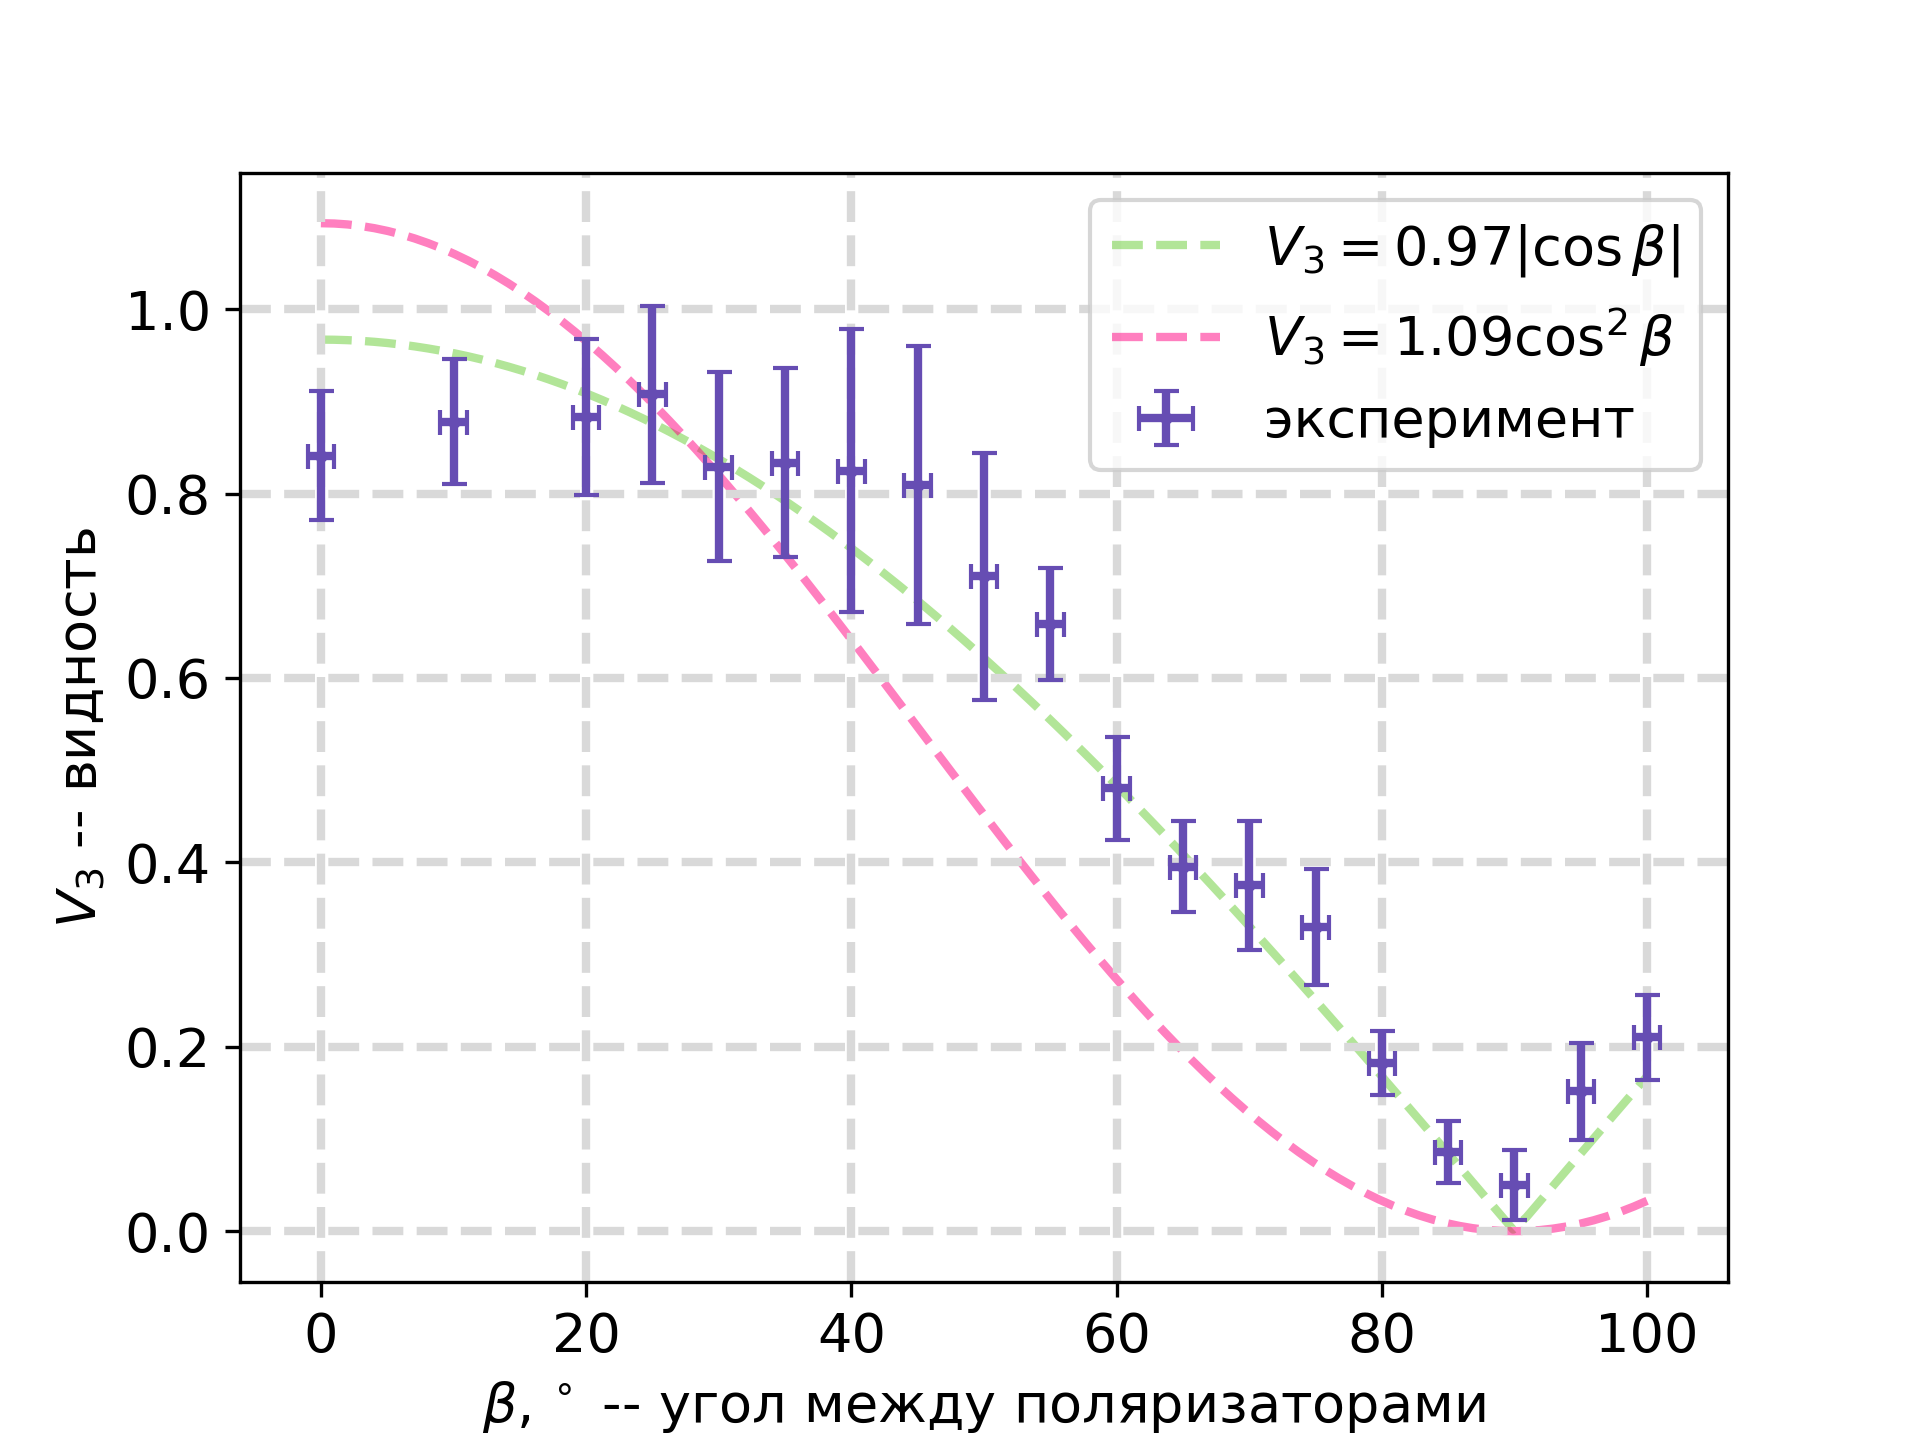
\includegraphics[width=\linewidth]{pics/graph1_nolin}
        \caption{Без линеаризации}
        \label{fig:graph1_nolin}
    \end{subfigure}
    \quad
    \begin{subfigure}[t]{0.35\linewidth}
        \centering
        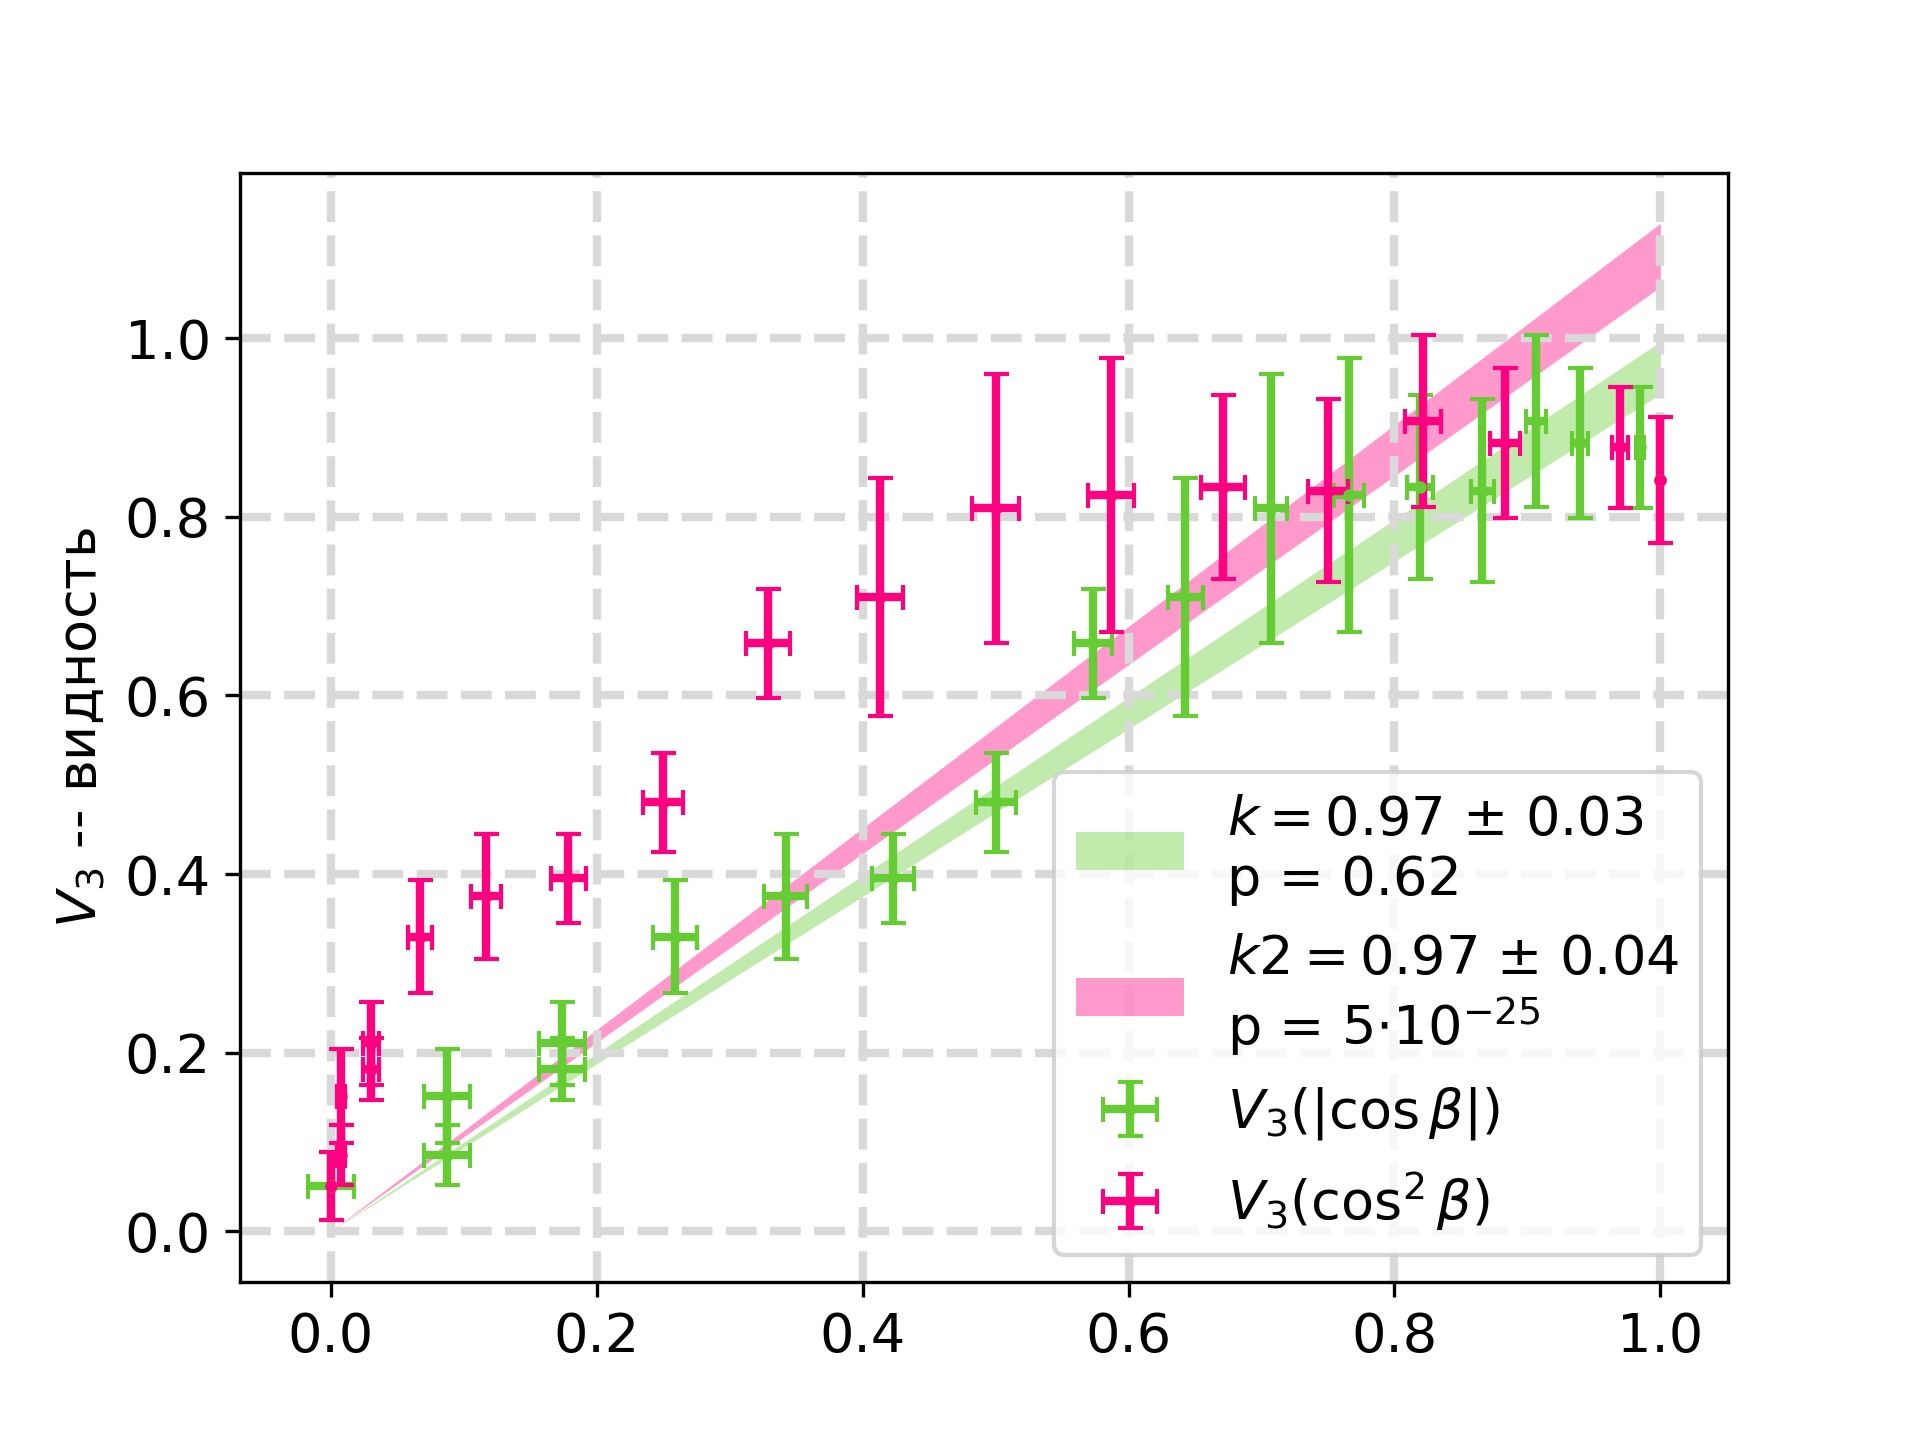
\includegraphics[width=\linewidth]{pics/graph1_lin}
        \caption{Линеаризации $V_3(|\cos\beta|)$ и $V_3(\cos^2\beta)$}
        \label{fig:graph1_lin}
    \end{subfigure}
\captionsetup{justification=raggedright, singlelinecheck=false}
    \caption{Измеренная зависимость видности от угла между\\поляроидами $V_3(\beta)$}
\end{figure}

Линеаризация \ref{fig:graph1_lin} позволяет видеть, что видность зависит от угла как $|\cos\beta|$. То есть \ul{лазерное излучение имеет постоянную линейную поляризацию}.

\clearpage

\section{Измерение зависимости видности от разности хода}

 \begin{wraptable}{r}{0.3\textwidth}
    \centering
    
\begin{tabular}{|c|c|c|}
\hline
\begin{tabular}[c]{@{}c@{}}$l$, см;   $\sigma_l = 1$ см\\ разность хода\end{tabular} & $V_2$ & $\sigma_{V_2}$ \\ \hline
-6                                                                                  & 0.76  & 0.12           \\ \hline
-1                                                                                  & 0.82  & 0.09           \\ \hline
0                                                                                   & 0.87  & 0.05           \\ \hline
6                                                                                   & 0.68  & 0.06           \\ \hline
12                                                                                  & 0.63  & 0.07           \\ \hline
18                                                                                  & 0.42  & 0.05           \\ \hline
24                                                                                  & 0.27  & 0.02           \\ \hline
30                                                                                  & 0.10  & 0.02           \\ \hline
36                                                                                  & 0.02  & 0.02           \\ \hline
42                                                                                  & 0.11  & 0.02           \\ \hline
48                                                                                  & 0.15  & 0.02           \\ \hline
54                                                                                  & 0.18  & 0.02           \\ \hline
60                                                                                  & 0.17  & 0.02           \\ \hline
66                                                                                  & 0.20  & 0.02           \\ \hline
72                                                                                  & 0.19  & 0.02           \\ \hline
78                                                                                  & 0.16  & 0.02           \\ \hline
84                                                                                  & 0.10  & 0.02           \\ \hline
90                                                                                  & 0.07  & 0.02           \\ \hline
96                                                                                  & 0.15  & 0.02           \\ \hline
102                                                                                 & 0.31  & 0.02           \\ \hline
108                                                                                 & 0.48  & 0.06           \\ \hline
114                                                                                 & 0.61  & 0.09           \\ \hline
120                                                                                 & 0.68  & 0.09           \\ \hline
126                                                                                 & 0.76  & 0.11           \\ \hline
132                                                                                 & 0.67  & 0.06           \\ \hline
\end{tabular}
\caption{Зависимость видности $V_3$ от разности хода $l$}
\label{tab:2}
\end{wraptable}

 В этом пункте начальное положение системы было выбрано так же, как и в прошлом. Теперь положение $\text{П}_2$ оставалось неизменным, но менялась координата блока $\text{Б}_2$ $x$. 

 В результате пересчета по формуле \eqref{eq:V2} была получена зависимость $V_2(l)$, где $l = 2 \Delta x$ -- разность хода лучей (1) и (2) в интерферометре Майкельсона. Результаты приведены в таблице \ref{tab:2} и на графике \ref{fig:graph2}.

 \begin{figure}[h]
    \raggedright
    
\includegraphics[width = 0.65\textwidth]{pics/graph2}
    \captionsetup{justification=raggedright, singlelinecheck=false}
    \caption{Зависимость видности от разности хода}
    \label{fig:graph2}
 \end{figure}

По периоду восстановления видности определена длина резонатора лазера $L = 63 \pm 6$ см и полуширина спада видности $l_{1/2} = 20 \pm 6$ см. По формулам \eqref{eq:assess} получена оценка ширины спектра излучения $\boxed{\Delta_nu = (0,9 \pm 0,3)\text{ ГГц}}$ и количества генерируемых мод $\boxed{n = 2,9 \pm 0,6}$. \ul{Полученная экспериментально спектральная ширина согласуется по порядку величины с допплеровским уширением спектра.}

\section{Заключение}

По итогам работы были сделаны выводы о поляризации и спектральном составе света, генерируемого исследуемым лазером. Поляризация оказалась постоянной линейной. Ширина спектра излучения $\Delta_nu = (0,9 \pm 0,3)\text{ ГГц}$ и количество генерируемых мод $n = 2,9 \pm 0,6$ согласуются с теоретическими оценками.

\end{document}